\documentclass[12pt, a4]{article}
\usepackage[left=20mm, top=20mm, right=15mm, bottom=20mm]{geometry}
\usepackage[utf8]{inputenc}
\usepackage{enumitem}
\usepackage{graphicx}
\usepackage{amssymb}
\usepackage{amsmath}
\usepackage{mathtools}
\usepackage{tocloft}
\usepackage[hidelinks, pdftex]{hyperref}
\usepackage[russian]{babel}

\title{КАНспекты}
\author{Матанализ}

\usepackage[nottoc]{tocbibind}
\setcounter{tocdepth}{5}

\setlength{\cftsubparaindent}{0.75cm}
\setlength\cftbeforesubparaskip{2.5pt}

\begin{document}

\begin{titlepage}
	\begin{center}
		\vspace*{5cm}

		\Huge
		\textbf{КАНСПЕКТЫ}

		\vspace{0.5cm}
		\LARGE
		матанблин
		
		\vfill
		
		
\includegraphics[scale=0.25]{koshka}
				
		\vfill
		
	\end{center}
\end{titlepage}

\renewcommand\contentsname{Ваши вопросы следующие:}
\tableofcontents
\vspace{2cm}
\texttt{
Что еще добавить?
\begin{itemize}
	\item мощности множеств, рац > нат и т.д.
	\item словами предел последовательности
	\item мб написать точки разрыва как в Кудрявцеве стр. 202-204
	\item Коши <=> Гейне
	\item ну и всякое, что было после интегралов: Ферма, Ла Гранж, Ролля и т.д.
\end{itemize}
}
\newpage

\subparagraph{Множество} --- одно из первичных понятий математикии, не требуещего своего определения. Это совокупность, собрание каких-либо объектов произвольной природы, мыслимых как единое целое. С множествами можно производить определенные операции по неким правилам, например, $\cap$ \textit{пересекать}, $\cup$ \textit{объединять}, $\setminus$ \textit{вычитать}, $\bigtriangleup$ вычислять \textit{симметрическую разность}, \textit{дополнять} и вычислять \textit{декартово прямое произведение}. \\
\\
Пусть даны множества $A = \{\textrm{\textit{с, т, у, д, е, н}}\}$, \ $B = \{\textrm{\textit{у, ч, е, н, и}}\}$, тогда:

\begin{itemize}
	\item пересечение $A\cap B = \{x \ | \ x\in A \ \wedge \ x\in B \}$ = \{\textrm{\textit{у, е, н}}\}
	\item объединение $A\cup B = \{x \ | \ x\in A \ \vee \ x\in B \}$  = \{\textrm{\textit{с, т, у, ч, д, е, н, и}}\}
	\item разность $A\setminus B = \{x \ | \ x\in A \ \wedge \ x\notin B \}$ = \{\textrm{\textit{с, т, д}}\}, \ $B\setminus A = \{x \ | \ x\in B \ \wedge \ x\notin A \}$ = \{\textrm{\textit{ч, и}}\}
	\item симметрическая разность $A \bigtriangleup B = \left( A \setminus B \right) \cup \left ( B \setminus A \right) = \left(A \cup B\right) \setminus \left(A \cap B\right) = \varnothing$ --- ($\varnothing$ только для данных $A$ и $B$ !)
	\item дополнение $C_{U}A = U\setminus A\equiv\{x\in U\mid x\not\in A\} = \{\textrm{\textit{а, б, в, г, ж, з, ..., м, о, п, р, ф, ..., я}}\}$, где $U$~---~универсальное множество (в данном случае --- русский алфавит)
\end{itemize}

\subparagraph{Декартово (прямое) произведение} двух множеств --- множество, элементами которого являются все возможные упорядоченные пары элементов исходных множеств. 
\[ X\times Y = \{(x, y) \ | \ x\in X, \ y\in Y \} \] 

Например:
\[ X = \{1, 2\}, \ Y = \{3, 4\} \] 
\[ X\times Y = \{(1, 3), (1, 4), (2, 3), (2, 4)\} \] 

\subparagraph{Свойство бесконечности (поглощение единицы)}
\[ |\mathbb{N}| + 1 = |\mathbb{N}| \] 

\subparagraph{Комплексное число} ($\mathbb{C}$) --- выражение вида 
\[x+iy, \ \textrm{где} \ x, y \in \mathbb{R}, \ \textrm{а} \ i \ \textrm{--- мнимая единица.} \] 

Комплексные числа можно \textit{складывать}, \textit{вычитать}, \textit{умножать}, \textit{делить}, но нельзя \textit{сравнивать}! Комплексное число отлично от нуля!
\[ |z| = \sqrt{x^2+y^2} \ \ \textrm{--- модуль комплексного числа} \]

\subparagraph{Функция} --- всякое однозначное отображение из одного множества в другое.

\subparagraph{Последовательность} --- функция из $\mathbb{N}$ в $\mathbb{R}$ или в $\mathbb{C}$.

\subparagraph{Метрическое пространство} --- непустое множество, в котором определены функции метрики:
\begin{enumerate}[leftmargin=2cm]
	\item $\rho(x, y) = 0 \ \Leftrightarrow \ x=y, \ \rho(x, y) \geq 0$ --- расстояние равно 0
	\item $\rho(x, y) = \rho(y, x)$ --- симметричность
	\item $\rho(x, z) \leq \rho(x, y) + \rho(y, z)$ --- неравенство треугольника
\end{enumerate}

Например:
\begin{itemize}[leftmargin=2cm]
	\item $\rho(x, y) = |y - x|$ --- метрика
	\item $\rho(x, y) = |x\cdot y|$ --- не метрика
	\item $\rho(x) = x^2$ --- некорректный пример
\end{itemize}

\subparagraph{Предел последовательности (по Коши)}

\[\forall \ \varepsilon>0 \ \ \exists \ \ N=N(\varepsilon) \in \mathbb{N}; \ \ \forall \ n>N \ \ |f_n-A|<\varepsilon \]

\subparagraph{Биекция}\mbox{}\\
\begin{minipage}{0.1\textwidth}
\end{minipage}
\hspace{0.5cm}
\begin{minipage}{0.6\textwidth}
	--- это такая функция отображения из множества $X$ в множество $Y$, при которой для каждого образа существует лишь \textbf{один} прообраз.
\end{minipage}
\hfill
\begin{minipage}{0.3\textwidth}
	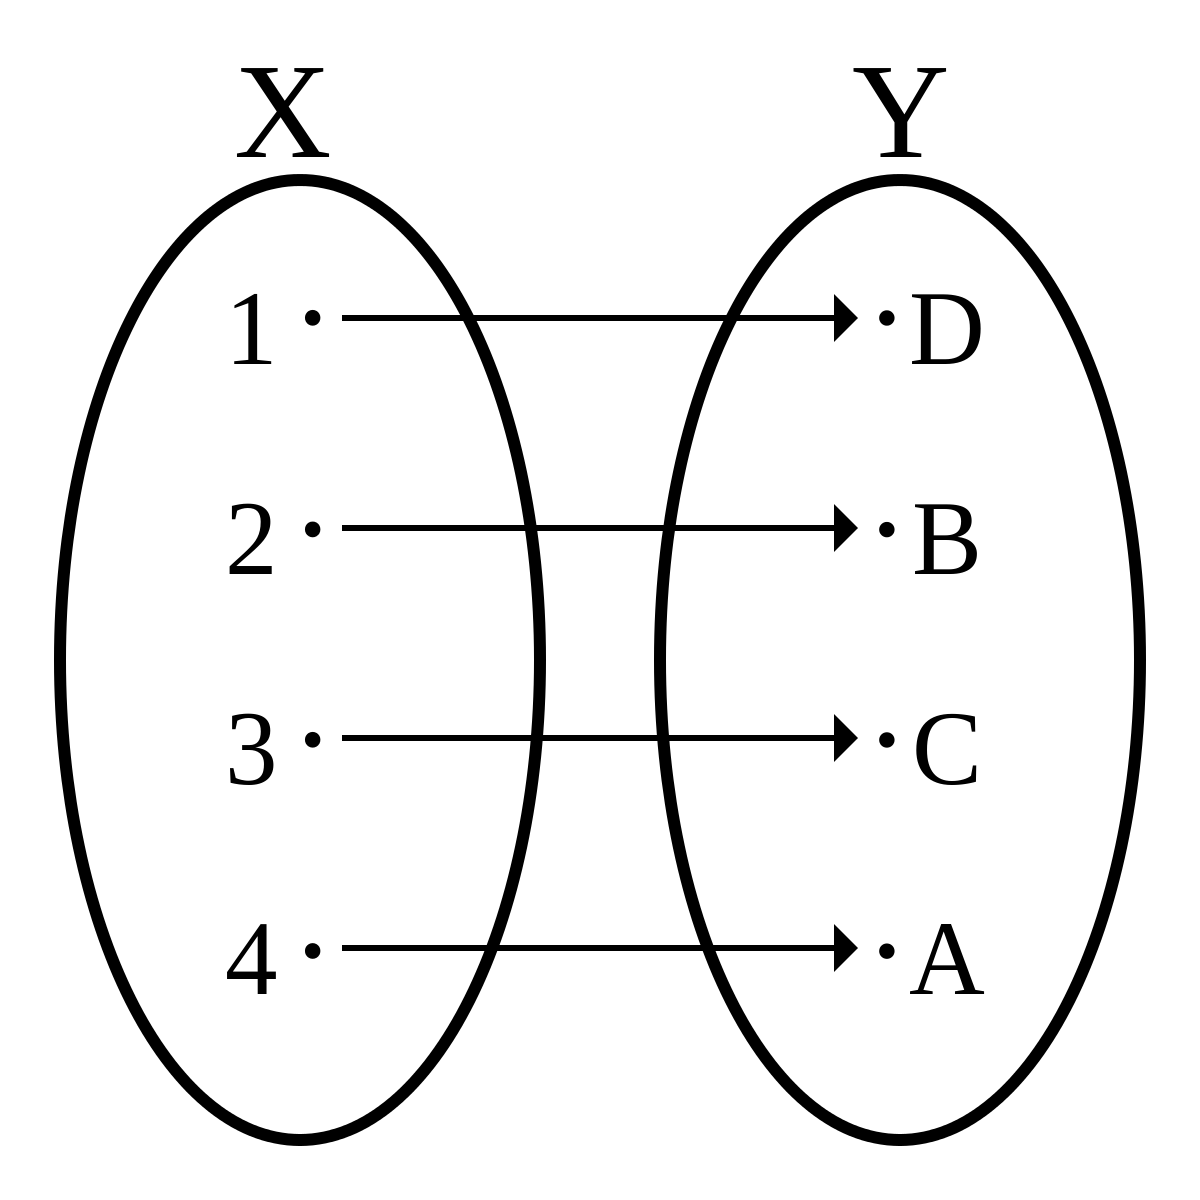
\includegraphics[scale=0.075]{biekcia}
\end{minipage}
\subparagraph{Инъекция}\mbox{}\\
\begin{minipage}{0.1\textwidth}
\end{minipage}
\hspace{0.5cm}
\begin{minipage}{0.6\textwidth}
	--- это такая функция отображения из множества $X$ в множество $Y$, при которой для каждого образа существует \textbf{не~более~одного} прообраза.
\end{minipage}
\hfill
\begin{minipage}{0.3\textwidth}
	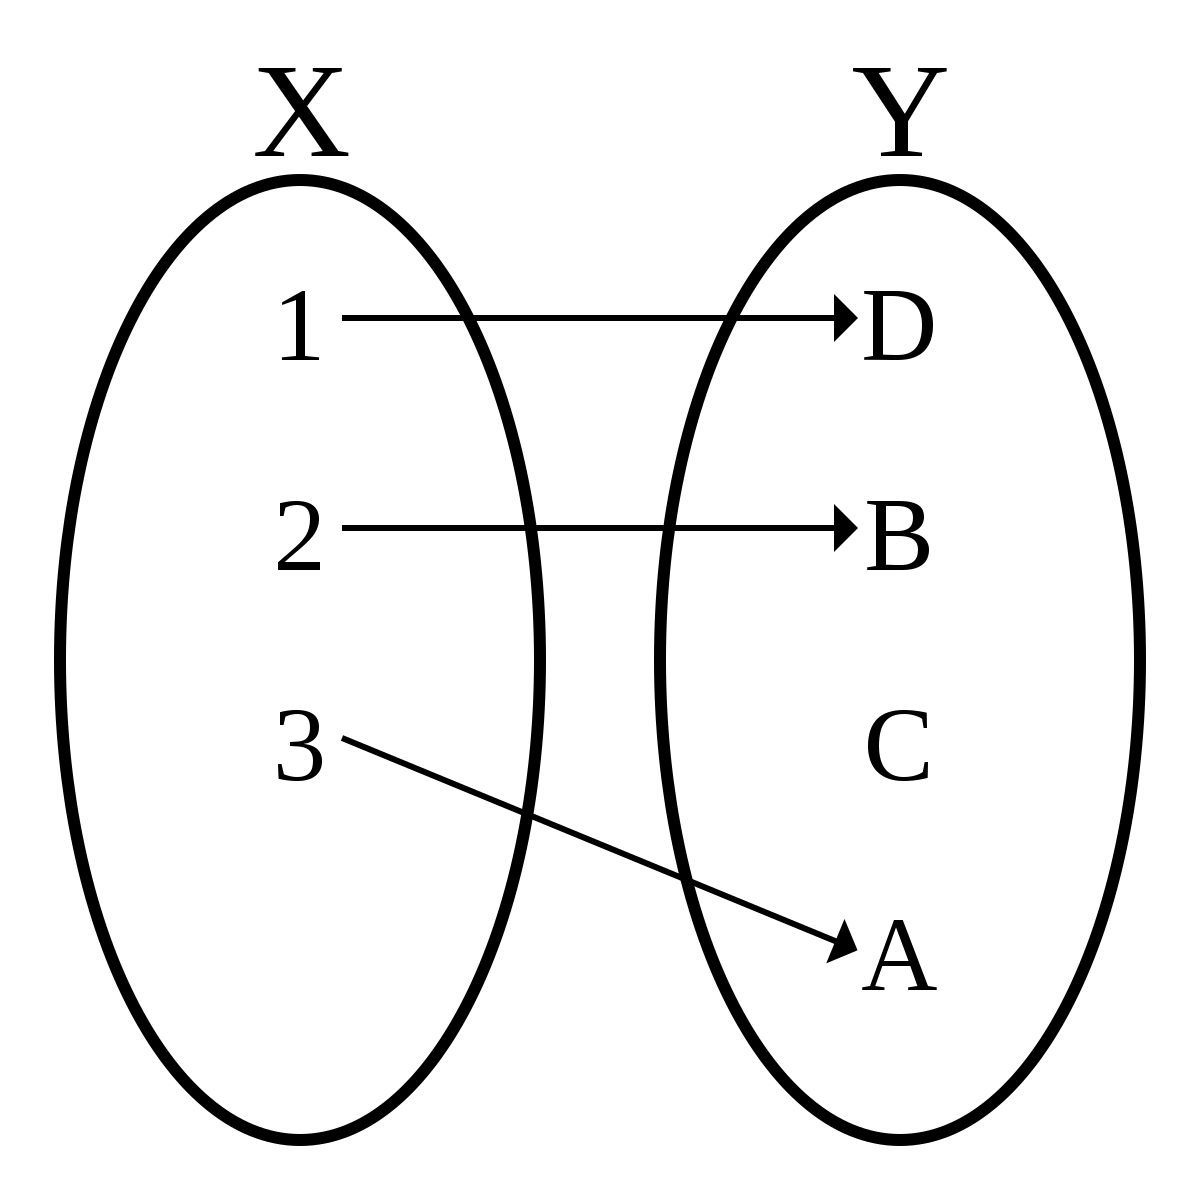
\includegraphics[scale=0.075]{injectia}
\end{minipage}
\subparagraph{Сюръекция}\mbox{}\\
\begin{minipage}{0.1\textwidth}
\end{minipage}
\hspace{0.5cm}
\begin{minipage}{0.6\textwidth}
	--- это такая функция отображения из множества $X$ в множество $Y$, при которой для каждого образа существует \textbf{не~менее~одного} прообраза.
\end{minipage}
\hfill
\begin{minipage}{0.3\textwidth}
	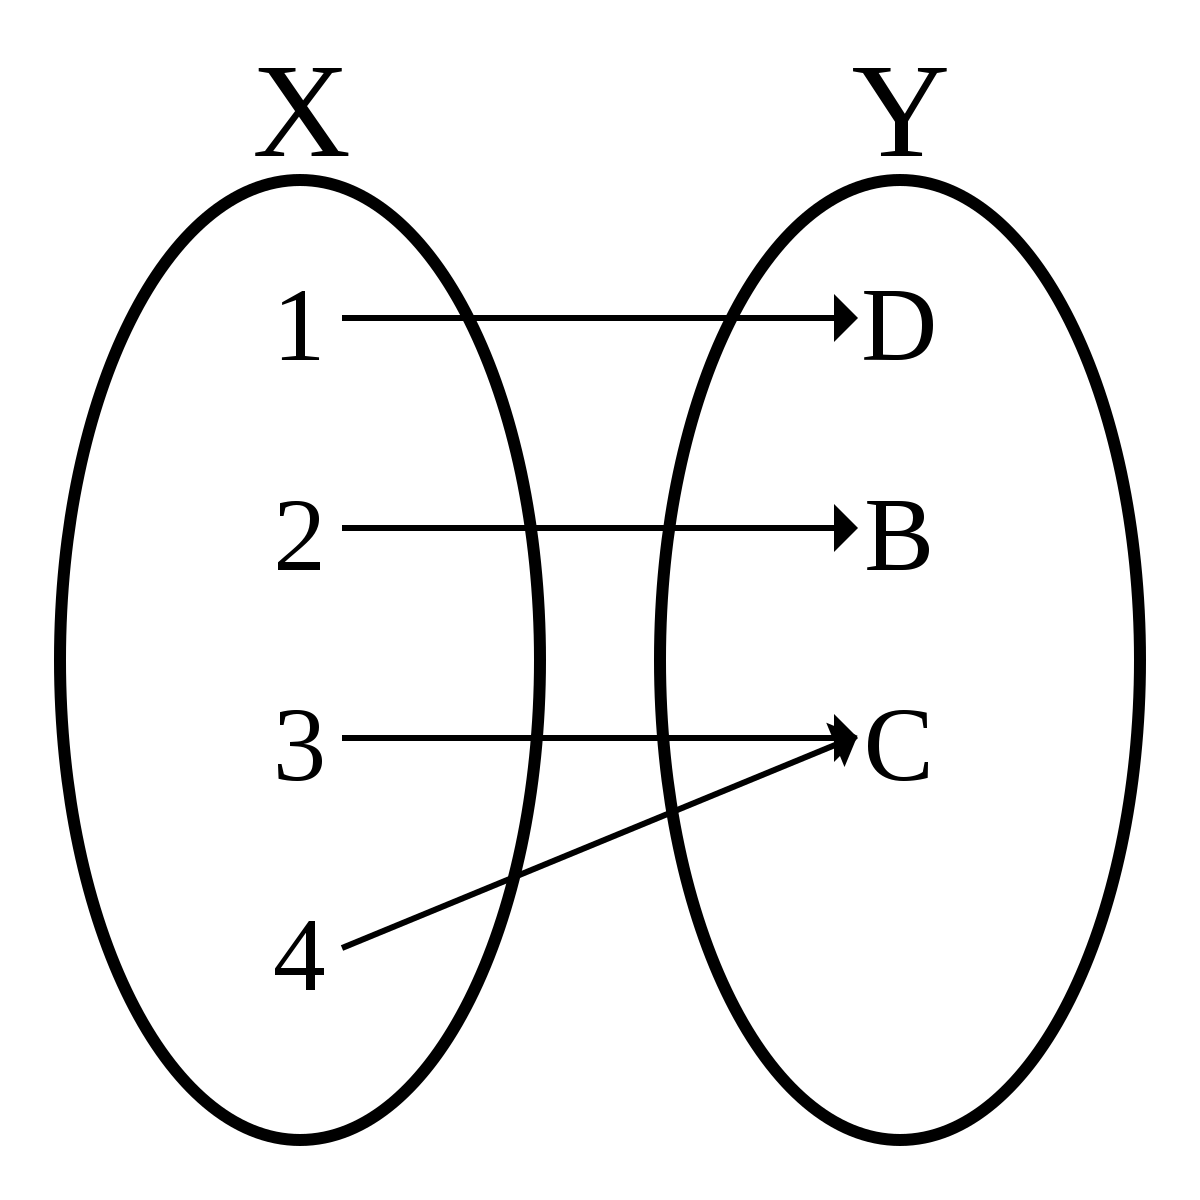
\includegraphics[scale=0.075]{surjectia}
\end{minipage}

\subparagraph{Первый замечательный предел} \mbox{}\\
\begin{minipage}{0.6\textwidth}
	\[\lim_{x\to 0}\frac{\sin(x)}{x} =1 \]
	\vfill
	\begin{center}
		следствия:
	\end{center}
	\[ \sin(x)\sim x \sim \arcsin(x) \sim \tg(x) \sim \arctg(x) \]
	\[ \cos(x) \sim 1 \]
	\vfill
\end{minipage}
\hfill
\begin{minipage}{0.4\textwidth}
		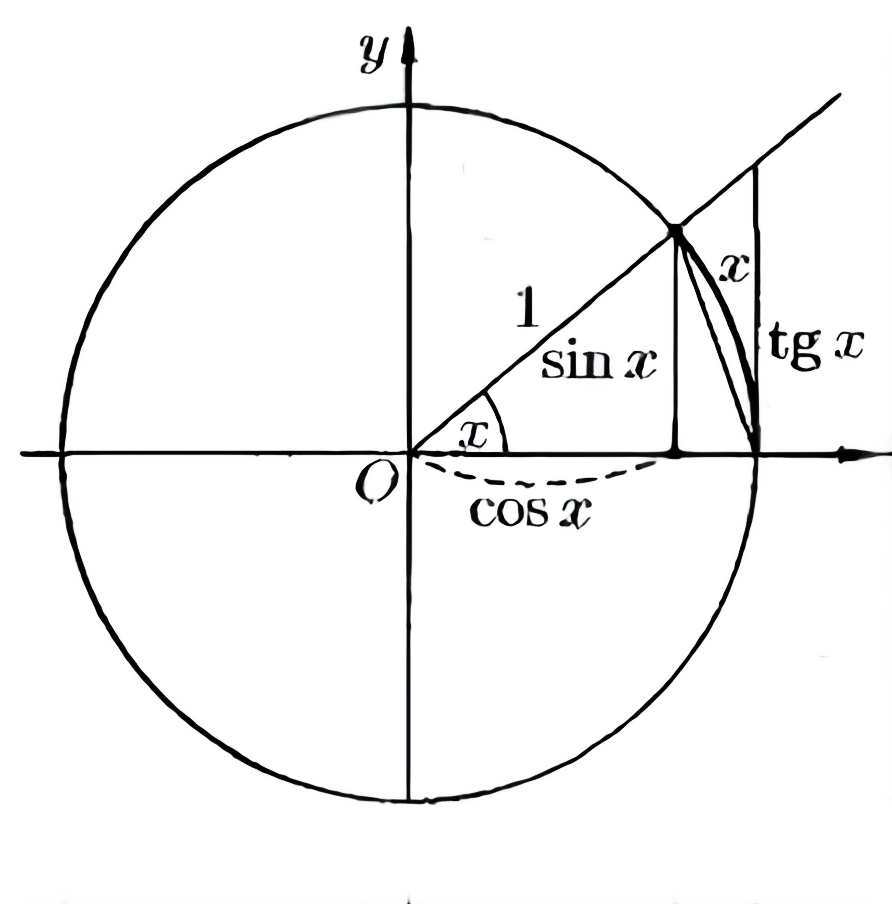
\includegraphics[scale=0.2]{1_predel_norm}
\end{minipage}

\subparagraph{Второй замечательный предел}

\[ \lim_{n\to \infty} (1+\frac{1}{n})^{n} = e \]

Следствия:
\begin{enumerate}[leftmargin=2cm]
	\item $\lim\limits_{u\to 0} (1+u)^{\frac{1}{u}} = e$
	
	\item $\lim\limits_{x\to 0} (1+\frac{k}{x})^{x} = e^k$
	
	\item $\lim\limits_{x\to 0} \frac{\ln(1+x)}{x} = 1$
	
	\item $\lim\limits_{x\to 0} \frac{e^x-1}{x} = 1$
	
	\item $\lim\limits_{x\to 0} \frac{a^x-1}{x\ln a} = 1$ для $a>0, \ a \neq 1$
	
	\item $\lim\limits_{x\to 0} \frac{(1+x)^{\alpha}-1}{\alpha x} = 1$
\end{enumerate}

\subparagraph{Неравенство Бернулли}
\[ (1+\alpha)^{n} \geqslant 1+n\alpha \ ,\textrm{ где} \ \alpha\geqslant-1, n \in \mathbb{N} \]

\subparagraph{Неравенство Коши}
\[ \sqrt[n]{a_1, ..., a_n} \geqslant \frac{a_1+...+a_n}{n} \ ,\textrm{ где}  \ a_1, ..., a_n>0\]

\subparagraph{Арифметическое пространство} --- такое метрическое пространство, в котором в качестве множества точек рассматривается множество строк длины $n$ из $\mathbb{R}$, а расстояние берётся евклидово.
\[ \mathbb{R}^{n} = \{(x_1, ..., x_n) \ | \ x_1, ..., x_n \in \mathbb{R} \} \]
\[ (\mathbb{R}^{n}, \ \rho(\vec{x}, \vec{y})) = \sqrt{(x_1-y_1)^2+...+(x_n-y_n)^2} \]

\subparagraph{Предел функции (по Коши)} --- число $A$ называется пределом функции $f(x)$ при $x\rightarrow x_0$, если для любого $\varepsilon>0$ существует зависящеее от него положительное число $\delta>0$ такое, что для любого $x$ из области определения функции $D(f)$ из неравенства $0<|x-x_0|<\delta$ следует неравенство $|f(x)-A|<\varepsilon$.

\[ A = \lim_{x\to x_0} f(x) \ \Leftrightarrow \ \forall \ \varepsilon>0 \ \ \exists \ \ \delta=\delta(\varepsilon)>0: \]
\[\forall \ x\in D(f) \ \textrm{из неравенства} \ 0<|x-x_0|<\delta \ \Rightarrow \ |f(x)-A|<\varepsilon \]

\subparagraph{Предел функции (по Гейне)} --- число $A$ называется пределом функции $f(x)$ при $x\rightarrow x_0$, если для любой последовательности аргументов $\{x_n\}^{\infty} _{n=1}$ выполняются 3 свойства:
\begin{equation*}
	\begin{rcases}
		\{x_n\}\subset D(f)
		\\
		x_n\rightarrow x_0,
		\\
		x_0 \notin \{x_n\}^{\infty} _{n=1}.
	\end{rcases}
	\Rightarrow
	\lim_{n\to \infty} f(x_n) = A 
\end{equation*}

\subparagraph{Производной} функции $f(x)$ в точке $x$ называется предел отношения приращения функции к приращению её аргумента, когда последний стремится к нулю, при условии, что этот предел существует и конечен.

\[ f'(x) = \lim_{\Delta x \to 0} \frac{f(x+\Delta x)-f(x)}{\Delta x} = \lim\limits_{{\Delta x}\to 0} \frac{\Delta{f(x)}}{\Delta x}. \]

\subparagraph{Формула Лейбница}

\[ (uv)^{(n)} = \sum_{k-0}^{n} C_{n}^{k} \cdot u^{(n-k)} \cdot v^{(k)} \ \textrm{, где } \ C_{n}^{k} = \frac{n!}{k! (n-k)!} \]

\subparagraph{Вычисление производной через логарифмы}
\[ y'=(\frac{\sqrt[4]{2x+3}\cdot\sqrt[5]{3x+4}}{(3x+5)^8}) \]
\begin{center}
	\fbox{$\ln a^n = n \ln a$}
\end{center}
\[ \ln y = \frac{1}{4}\ln(2x+3) + \frac{1}{5}\ln(3x+4) - 8\ln(3x+5) \]
\begin{center}
	\fbox{$y' = y\cdot(\ln y)'$}
\end{center}
\[ \frac{y'}{y} = (\ln y)' = \frac{1}{4}\cdot\frac{2}{2x+3} + \frac{1}{5}\cdot\frac{3}{3x+4} - 8\cdot\frac{3}{3x+5} \]

\[\Rightarrow \ y' = (\frac{1}{4x+6} + \frac{3}{15x+20} - \frac{24}{3x+5}) \cdot \frac{\sqrt[4]{2x+3}\cdot\sqrt[5]{3x+4}}{(3x+5)^8} \]
\\
для $(x^x)'$:
\[ (x^x)' = (y)' = y(\ln y)' = x^x(\ln x^x)' = x^x(x\ln x)' = x^x(1+\ln x) \]
\\
для $(x^{x^x})'$:
\[ (x^{x^x})' = (y)' = x^{x^x}(x^{x}\ln x)' = x^{x^x}(x^x(1+\ln x)\cdot \ln x + x^{x-1}) \]

\subparagraph{Точка разрыва 1-го рода} --- точка, в которой нарушено условие непрерывности функции, в которой существуют и конечны оба односторонних предела 1-го рода.

\subparagraph{Точка разрыва 2-го рода} \mbox{}\\
\begin{minipage}{0.1\textwidth}
\end{minipage}
\hspace{0.5cm}
\begin{minipage}{0.6\textwidth}
	--- точка, в которой хотя бы один из двух односторонних пределов 1-го рода не существует либо равен $\infty$.
\end{minipage}
\hfill
\begin{minipage}{0.3\textwidth}
	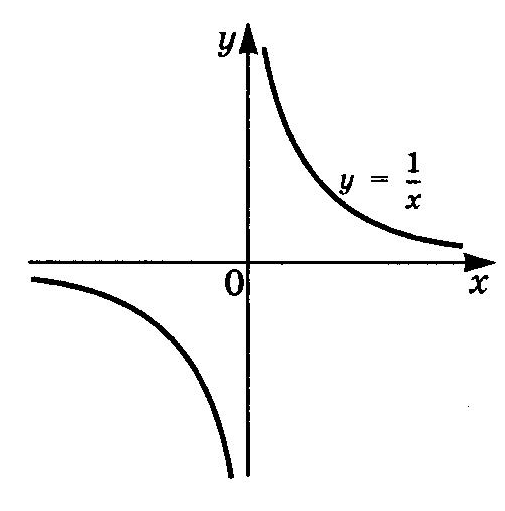
\includegraphics[scale=0.25]{razryv_2_rod}
\end{minipage}

\subparagraph{Устранимый разрыв} --- если существуют левый и правый пределы функции $f(x)$ в точке, и они равны, но не совпадают со значанием функции в точке $a$, или точка $a$ не определена, то точка $a$ называется точкой устранимого разрыва.

\subparagraph{Неопределенный интеграл} --- множество всех тех функций, производная которых равна заданной функции.

\subparagraph{Дифференциал функции} --- часть её приращения, главная и линейная по приращению аргумента, который стремится к нулю.

\[ d(f(x)) = f(x)'dx \]
\[ \Rightarrow f'(x) = \frac{d(f(x))}{dx} \]

дифференциал 2-го порядка:

\[ d^2(y) = d(dy) = d(f'(x)dx) = (f'(x)dx)'dx = [((f'(x))'dx + f'(x)(dx)']dx = \] \[= (f''(x)dx)dx = f''(x)\cdot(dx)^2\]

\[\Rightarrow d^2(y) = f''(x)\cdot(dx)^2\]

дифференциал $n$-го порядка:

\[d^{n}(y) = f^{(n)}(x)\cdot(dx)^{n}\]
 


\end{document}